\documentclass[conference]{IEEEtran}
\IEEEoverridecommandlockouts
\usepackage{cite}
\usepackage{amsmath,amssymb,amsfonts}
\usepackage{algorithmic}
\usepackage{graphicx}
\usepackage{textcomp}
\usepackage{xcolor}
\usepackage{booktabs}
\usepackage{float}
\usepackage{url}
\usepackage[caption=false,font=footnotesize]{subfig}
\usepackage{placeins}

\def\BibTeX{{\rm B\kern-.05em{\sc i\kern-.025em b}\kern-.08em
T\kern-.1667em\lower.7ex\hbox{E}\kern-.125emX}}

\begin{document}

\title{Reinforcement-Learning-Based Adaptive Locomotion Control for a Quadruped Robot on Rough Low-Friction Terrain}
\author{Tianyi Guan \quad Hanyu Wang\\
Yuanpei College, Peking University\\
2400017423@stu.pku.edu.cn}

\maketitle

\begin{abstract}
Quadruped locomotion on rough and low-friction terrain requires the controller to handle high-dimensional robot dynamics, intermittent contacts, terrain-dependent foot placement, and balance recovery at the same time. This course project builds a MuJoCo-based reinforcement learning pipeline for a Unitree A1 quadruped robot. The system first uses terrain raycasting and Jacobian-based inverse kinematics to initialize a physically plausible standing pose, avoiding floating or ground penetration at reset. It then trains PPO policies for standing recovery and walking. To improve the realism of the walking gait, behavior cloning from a dog-trot motion clip is used to obtain a natural gait prior, and the PPO fine-tuning stage uses a frozen behavior-cloned policy as a teacher to regularize the action distribution. The intended final system is a hierarchical controller: a lightweight state classifier detects whether the robot should continue walking or switch to the recovery policy after a disturbance. Experiments show that the learned walking policy can walk on both the training wave terrain and a more irregular heightfield. Under lower friction and stronger terrain perturbation, the robot remains stable but becomes more conservative in speed.
\end{abstract}

\section{Introduction}
Quadruped robots have better terrain traversal capability than wheeled robots because they can use discrete footholds and actively regulate body posture. In real environments, however, the ground is rarely flat and high-friction. Grass, slopes, soft soil, gravel, and icy surfaces all change the contact condition between the feet and the terrain. Robust quadruped locomotion is therefore difficult because the system contains a floating base, twelve actuated joints, nonlinear rigid-body dynamics, and multiple intermittent contacts. The problem becomes even harder on rough and low-friction terrain, where foot slip and sudden height changes can easily destabilize the robot.

Traditional quadruped locomotion controllers often rely on manually designed gait schedules, swing-foot trajectories, inverse kinematics, and low-level PD or impedance controllers. These methods are interpretable and efficient, but their performance is highly dependent on hand-designed assumptions about terrain geometry, friction, and contact timing. When the environment changes significantly, the controller may need to be redesigned or heavily retuned. Reinforcement learning provides a complementary approach: instead of explicitly designing every motion primitive, a policy can learn closed-loop behavior from physical simulation and task rewards.

In this project, we use the Unitree A1 robot model in MuJoCo and formulate recovery and walking as continuous-control reinforcement learning problems. The policy outputs 12 normalized joint target offsets. These targets are tracked by MuJoCo position actuators, which approximate a PD joint control layer. This design reduces the difficulty of learning compared with direct torque control. The pipeline includes terrain-aware standing initialization, PPO-based recovery and walking policies, behavior-cloning pretraining from a reference trot motion, and PPO fine-tuning with a frozen teacher-policy regularization term. The final goal is not only to train isolated recovery and walking skills, but also to connect them with a small classifier so that the robot can autonomously choose when to walk and when to recover.

\section{Related Work}
Classical legged locomotion control is usually decomposed into gait planning, foot trajectory generation, inverse kinematics, and stability control. A gait planner specifies the stance and swing phases of each leg; a foot trajectory generator defines desired swing-foot clearance and landing locations; inverse kinematics maps desired foot positions to joint targets; and a low-level controller tracks these joint or torque commands. This decomposition is closely related to the motion planning, kinematics, and motion control topics covered in the course.

Deep reinforcement learning has become a common tool for learning locomotion policies in simulation. PPO is widely used because of its relative stability and simplicity for continuous-control tasks~\cite{ppo}. Hwangbo et al. showed that reinforcement learning can train agile and dynamic motor skills for legged robots and transfer them to real hardware~\cite{hwangbo2019learning}. Lee et al. extended learning-based quadruped locomotion to more challenging terrain conditions~\cite{lee2020learning}. Kumar et al. proposed rapid motor adaptation (RMA) on a Unitree A1 robot, emphasizing real-time adaptation to changing dynamics and terrain properties~\cite{kumar2021rma}. Margolis et al. further demonstrated the potential of reinforcement learning for rapid locomotion~\cite{margolis2022rapid}. A recent systematic review also points out that reward design, policy representation, and training stability remain major challenges for DRL-based legged locomotion~\cite{sun2024systematic}.

However, pure task-reward optimization can produce unnatural behaviors, such as high-frequency joint jitter, tiny sliding steps, or asymmetric gaits that exploit the reward design. Motion imitation offers a way to introduce a more natural locomotion prior. The work by Peng, Coumans, et al. learns agile locomotion skills by imitating reference animal motions, using reward terms that track joint pose, joint velocity, end-effector motion, root pose, and root velocity~\cite{peng2020learning}.

This project follows the same general motivation but uses a lighter implementation. Instead of building a full reference-trajectory imitation reward during PPO, I first train a behavior-cloned policy from a dog-trot motion clip and then use this frozen policy as a teacher during PPO fine-tuning. The teacher reward penalizes large deviations from the behavior-cloned action distribution, which helps prevent PPO from forgetting the natural gait prior.

\section{Problem Formulation}
Both the recovery and walking tasks are modeled as finite-horizon Markov decision processes
\begin{equation}
\mathcal{M}=(\mathcal{S}, \mathcal{A}, P, r, \gamma).
\end{equation}
The state $s_t \in \mathcal{S}$ is represented by proprioceptive observations and, for walking, a gait clock. The basic observation includes trunk orientation, base velocity, angular velocity, 12 joint positions, 12 joint velocities, and the previous action. For walking, the observation also includes $\sin(\phi)$, $\cos(\phi)$, the target forward velocity, and the desired contact pattern of the four feet. For recovery, the reset distribution includes easier upright perturbations as well as harder side-lying or upside-down configurations, so that the policy learns to stand up from disturbed poses rather than only maintain an already stable posture.

The action $a_t \in [-1,1]^{12}$ is a normalized joint target offset. The actual target joint configuration is
\begin{equation}
q^{\mathrm{tar}}_t =
\mathrm{clip}(q^{\mathrm{stand}}_t + \alpha a_t, q_{\min}, q_{\max}),
\end{equation}
where $q^{\mathrm{stand}}_t$ is the terrain-aware nominal standing posture, $\alpha$ is the action scale, and $q_{\min}, q_{\max}$ are joint limits. MuJoCo position actuators then track $q^{\mathrm{tar}}_t$, which acts as a low-level PD-like controller.

The reinforcement learning objective is to maximize the expected discounted return:
\begin{equation}
\max_{\pi_\theta} \mathbb{E}_{\pi_\theta}
\left[\sum_{t=0}^{T-1}\gamma^t r(s_t,a_t)\right].
\end{equation}
For recovery, the reward mainly encourages upright trunk orientation, reasonable body height, low joint velocity, smooth actions, and non-catastrophic contact behavior. For walking, the task reward contains forward-velocity tracking, progress, uprightness, body-height tracking, gait-contact matching, swing-foot clearance, lateral drift penalty, yaw-rate penalty, pitch/roll tilt penalty, joint-velocity penalty, action penalty, smoothness penalty, stance-foot slip penalty, insufficient-support penalty, and fall penalty.

To reduce gait forgetting during PPO fine-tuning, I add a teacher action reward:
\begin{equation}
r_{\mathrm{teacher}} =
w_{\mathrm{bc}}\exp\left(-k_{\mathrm{bc}}
\|a_t-a^{\mathrm{teacher}}_t\|_2^2/d_a\right),
\end{equation}
where $a^{\mathrm{teacher}}_t$ is the deterministic action predicted by the frozen behavior-cloned policy under the same normalized observation, and $d_a=12$ is the action dimension. The final reward is
\begin{equation}
r_t = r_{\mathrm{task}} + r_{\mathrm{teacher}} - r_{\mathrm{penalty}}.
\end{equation}

For the integrated anti-disturbance system, the high-level controller can be viewed as a discrete policy selector
\begin{equation}
m_t = c_\psi(s_t) \in \{\mathrm{walk}, \mathrm{recover}\},
\end{equation}
where $c_\psi$ is a lightweight classifier or rule-based state estimator. The executed action is then
\begin{equation}
a_t =
\begin{cases}
\pi_{\mathrm{walk}}(s_t), & m_t=\mathrm{walk},\\
\pi_{\mathrm{recover}}(s_t), & m_t=\mathrm{recover}.
\end{cases}
\end{equation}
The classifier uses posture and contact-related features such as trunk uprightness, body height, angular velocity, foot support count, and recent fall indicators. This formulation separates skill learning from mode selection: PPO learns specialized low-level skills, while the classifier handles when each skill should be activated.

\section{Method}
\subsection{System Overview}
The project is organized as a standard simulation-to-learning pipeline. The MuJoCo XML model defines the Unitree A1 body, joints, actuators, collision geoms, and heightfield terrain. A Gymnasium environment wraps MuJoCo states and exposes a continuous action space. Stable-Baselines3 PPO is used for policy optimization, and Weights \& Biases is used for logging training metrics. The demo scripts load saved checkpoints and VecNormalize statistics to inspect policies in the interactive MuJoCo viewer or export videos.

The development process followed the same order as the presentation. First, we built a physically reasonable baseline that can stand on uneven terrain and slide downhill under low friction without artificial motion commands. Second, we trained recovery policies that can return from disturbed poses to a stable standing state. Third, we trained walking policies and found that task-only PPO easily produced small high-frequency steps. Finally, we added imitation learning and teacher regularization to make the walking behavior more natural.

The next system-level step is to combine the two skills through a policy-switching controller. During normal locomotion, the walking checkpoint is used. If the classifier detects that the robot has lost balance, is too low, has very low uprightness, or has abnormal angular velocity, control is transferred to the recovery checkpoint. Once the robot returns to a stable upright state, the controller switches back to the walking checkpoint. In implementation, hysteresis or a minimum dwell time should be added to avoid rapid oscillation between the two policies near the decision boundary.

\subsection{Terrain-Aware Standing Initialization}
An early issue in the demo was that the robot could start with its feet penetrating the terrain or with the body floating above the map. To make the initial state physically meaningful, the environment estimates local terrain height using raycasting. It queries the terrain height under the base and near each foot, then constructs target foot positions that match the local ground height. A Jacobian-based inverse kinematics solver computes joint angles that place the feet near these target positions while keeping the trunk at a reasonable height. After this step, a collision-based lifting procedure ensures that the robot is not initialized inside the terrain.

This initialization is important because the policy should learn from realistic contacts rather than artifacts caused by an invalid reset pose. It also helps the robot stand on uneven terrain without simply shifting the whole body upward by a fixed amount.

One limitation is that the current inverse-kinematics solution is not perfectly symmetric between the front and rear legs. Because the A1 mechanical structure and the local IK targets are not exactly symmetric, the robot can show different passive sliding trajectories when rotated by 180 degrees on a low-friction slope. This observation was useful during debugging: it showed that apparent downhill motion is affected not only by gravity and terrain, but also by the initial contact geometry produced by IK.

\subsection{Recovery Curriculum}
Before training the walking policy, we trained recovery behavior from randomized initial poses. A curriculum was used to avoid exposing PPO to very hard resets at the beginning. The early stage samples small perturbations around the standing pose. As training progresses, the reset distribution gradually includes larger body orientation errors, lower trunk height, stronger joint perturbations, and higher initial velocities. This makes the policy first learn basic balance and then learn to recover from side-lying or heavily disturbed poses.

The current recovery policy has visibly better stand-up behavior than the zero-action baseline, but difficult states remain challenging. In particular, when the initial uprightness is very low, the trunk is close to the ground, or the initial joint/velocity perturbation is large, recovery can still fail. This reflects the high exploration difficulty of recovery: the policy must discover coordinated leg motions while avoiding self-collision and invalid contacts.

\subsection{Gait Clock and Walking Reward}
The walking environment uses a gait clock to define a diagonal trot pattern. The leg order is FR, FL, RR, RL, and the phase offsets are
\begin{equation}
\phi_{\mathrm{offset}} = [0,\pi,\pi,0].
\end{equation}
This means that FR/RL and FL/RR form two alternating diagonal pairs. The reward encourages stance feet to stay near the ground and avoid horizontal slip, while swing feet should lift above the terrain with enough clearance. The environment also penalizes insufficient support, missing stance contacts, and cases where both rear feet lose support. These terms reduce unrealistic behaviors such as hopping with the rear legs lifted or sliding forward with tiny foot motions.

\subsection{Behavior-Cloning Pretraining}
The behavior-cloning stage uses a dog-trot motion clip from the motion imitation dataset. Since the reference animal motion and the MuJoCo A1 model do not share exactly the same joint offsets and proportions, I use centered retargeting. The cyclic variation of the reference motion is preserved, but its mean joint configuration is aligned with the A1 terrain-aware standing posture. The expert action is computed as the joint target offset required to track the retargeted reference joint angles.

The behavior-cloning loss is
\begin{equation}
\mathcal{L}_{\mathrm{BC}} =
\frac{1}{N}\sum_{i=1}^{N}
\|\mu_\theta(o_i)-a^{\mathrm{expert}}_i\|_2^2,
\end{equation}
where $\mu_\theta(o_i)$ is the actor mean action. The current BC checkpoint is stored under \verb|runs/walk_bc_dog_trot_v3| and is used as the teacher for later PPO fine-tuning.

\subsection{PPO Fine-Tuning with a Frozen Teacher}
Directly fine-tuning the BC policy with PPO caused the policy to forget the natural trot prior and sometimes converge to less realistic behaviors. To address this, I added a wrapper around the walking environment. Each environment worker loads the frozen BC policy and its saved observation normalization statistics. At every step, the wrapper computes the teacher action for the current raw observation, compares it with the PPO action, and adds the exponential teacher reward described above.

This design keeps PPO flexible: it can still improve speed tracking and stability using the task reward, but large deviations from the teacher gait are discouraged. In practice, this helped reduce catastrophic gait drift during PPO fine-tuning. On macOS, loading a frozen PyTorch/SB3 teacher inside \verb|SubprocVecEnv| is not safe with the \verb|fork| start method, so the training script automatically switches to \verb|forkserver| when teacher regularization is enabled with multiple environments.

This teacher-regularized route directly follows the ``next step'' described in the presentation: first obtain a more realistic walking prior on easier terrain through imitation learning, then use PPO to adapt that prior to the low-friction rough-terrain setting.

\section{Experiments}
\subsection{Experimental Setup}
The simulation uses MuJoCo 3.x and the Unitree A1 model. The policy is a Stable-Baselines3 PPO MLP policy with two hidden layers of size 256 for both the actor and the critic. The action dimension is 12. The main training terrain is a $6\mathrm{m}\times6\mathrm{m}$ wave heightfield. For generalization testing, we created an additional irregular heightfield with random bumps, depressions, and multi-frequency terrain variations. We also reduced the terrain friction to test whether the policy remains stable when foot slip becomes more likely.

\begin{figure}[htbp]
\centering
\subfloat[Wave terrain\label{fig:terrain-wave}]{
  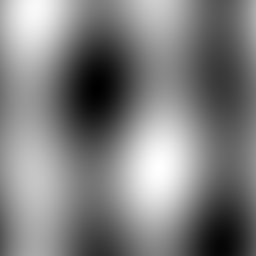
\includegraphics[width=0.46\linewidth]{terrain_wave.png}}
\hfill
\subfloat[Irregular terrain\label{fig:terrain-irregular}]{
  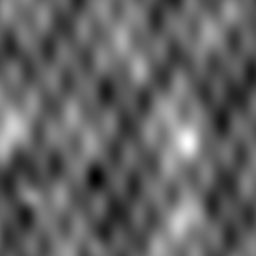
\includegraphics[width=0.46\linewidth]{terrain_irregular.png}}
\caption{Heightfields used in the walking benchmark. Brighter pixels represent higher terrain.}
\label{fig:terrain}
\end{figure}

The walking benchmark compares two checkpoints: the behavior-cloned trot policy in \verb|runs/walk_bc_dog_trot_v3| and the teacher-regularized PPO policy in \verb|runs/walk_after_bc_teacher_v1|. Evaluation uses the deterministic policy, a maximum episode length of 500 policy steps, a target velocity of $0.2\mathrm{m/s}$, and a gait frequency of $1.2\mathrm{Hz}$. For each checkpoint--terrain--friction combination, 10 episodes are evaluated. The raw benchmark outputs are stored in \verb|runs/walk_benchmark_checkpoint_scene_friction_v1|.

Because raw episode return is affected by episode length, especially when a policy falls early, I also report a regularized reward metric:
\begin{equation}
\bar{r}_{\mathrm{step}}=\frac{R_{\mathrm{episode}}}{N_{\mathrm{step}}},
\end{equation}
and a min-max normalized version of this per-step reward across all benchmark conditions. This makes the reward comparison less dominated by survival time and more suitable for comparing policy quality under controlled terrain and friction settings.

\subsection{Progress and Generalization Results}
The current demo results match the presentation observations. The terrain-aware baseline can stand on the heightfield without obvious penetration. Under low friction, passive motion is mainly caused by physical contact and gravity rather than a manually scripted sliding command. The recovery policy shows clear attempts to return to a standing posture after disturbances, although extremely low initial uprightness and severe pose perturbations are still difficult.

For walking, the early PPO-only policy could move forward on low-friction uneven terrain, but the visual gait was not fully realistic: it tended to use small, high-frequency corrective steps. After adding behavior cloning and teacher-regularized PPO, the walking motion became more stable and more aligned with the reference trot prior. Table~\ref{tab:walk-benchmark} gives a larger benchmark across checkpoints, scenes, and friction values.

To make the benchmark easier to interpret, I also visualize each setting as a normalized performance profile. The four axes are survival rate, forward-velocity score, normalized per-step reward, and lateral-stability score. Larger values are better on all axes. Figures~\ref{fig:profile-by-terrain}--\ref{fig:profile-by-checkpoint} present the same benchmark from three controlled-variable views: fixed terrain, fixed friction, and fixed checkpoint.


The benchmark shows three main observations. First, the behavior-cloned checkpoint is able to survive on the original wave terrain, but its speed is low and it fails to generalize to the irregular heightfield: the survival rate drops to 10--40\% and the mean forward velocity can become negative. This suggests that behavior cloning alone captures a trot-like motion prior but does not provide sufficient closed-loop robustness. Second, the teacher-regularized PPO checkpoint survives all evaluated walking settings. On the original wave terrain, it maintains a velocity close to the target speed. Third, on irregular and low-friction terrain, the PPO policy remains stable but becomes conservative; the mean forward velocity drops to about $0.08$--$0.10\mathrm{m/s}$ and the average height error increases. This agrees with the presentation's conclusion that the current walking reward still does not directly constrain stride length, cadence, and gait morphology strongly enough.

\begin{table*}[htbp]
\caption{Walking Benchmark with Per-Step Reward Normalization}
\label{tab:walk-benchmark}
\centering
\scriptsize
\begin{tabular}{llcccccc}
\toprule
Checkpoint & Terrain & Fric. & Survival & Mean vel. & Reward/step & Norm. reward & $|h_{\mathrm{err}}|$ \\
\midrule
BC trot & Wave h=0.30 & 1.0 & 10/10 & 0.074 & 5.95 & 0.71 & 0.016 \\
BC trot & Wave h=0.30 & 0.8 & 10/10 & 0.101 & 6.60 & 0.85 & 0.016 \\
BC trot & Wave h=0.30 & 0.7 & 10/10 & 0.119 & 6.94 & 0.93 & 0.016 \\
BC trot & Irregular h=0.30 & 1.0 & 3/10 & -0.028 & 3.10 & 0.06 & 0.015 \\
BC trot & Irregular h=0.30 & 0.8 & 3/10 & -0.039 & 3.97 & 0.26 & 0.013 \\
BC trot & Irregular h=0.30 & 0.7 & 4/10 & -0.013 & 3.44 & 0.14 & 0.013 \\
BC trot & Irregular h=0.40 & 1.0 & 2/10 & 0.003 & 3.82 & 0.23 & 0.006 \\
BC trot & Irregular h=0.40 & 0.8 & 1/10 & -0.051 & 2.82 & 0.00 & 0.005 \\
BC trot & Irregular h=0.40 & 0.7 & 3/10 & -0.018 & 4.23 & 0.32 & 0.005 \\
\midrule
Teacher PPO & Wave h=0.30 & 1.0 & 10/10 & 0.188 & 7.24 & 1.00 & 0.070 \\
Teacher PPO & Wave h=0.30 & 0.8 & 10/10 & 0.186 & 7.26 & 1.00 & 0.071 \\
Teacher PPO & Wave h=0.30 & 0.7 & 10/10 & 0.185 & 7.24 & 1.00 & 0.070 \\
Teacher PPO & Irregular h=0.30 & 1.0 & 10/10 & 0.098 & 6.48 & 0.82 & 0.132 \\
Teacher PPO & Irregular h=0.30 & 0.8 & 10/10 & 0.098 & 6.49 & 0.83 & 0.132 \\
Teacher PPO & Irregular h=0.30 & 0.7 & 10/10 & 0.092 & 6.49 & 0.83 & 0.132 \\
Teacher PPO & Irregular h=0.40 & 1.0 & 10/10 & 0.087 & 6.24 & 0.77 & 0.143 \\
Teacher PPO & Irregular h=0.40 & 0.8 & 10/10 & 0.084 & 6.25 & 0.77 & 0.142 \\
Teacher PPO & Irregular h=0.40 & 0.7 & 10/10 & 0.081 & 6.24 & 0.77 & 0.142 \\
\bottomrule
\end{tabular}
\end{table*}
\FloatBarrier

\begin{figure}[H]
\centering
\subfloat[Wave h=0.30\label{fig:profile-wave}]{
  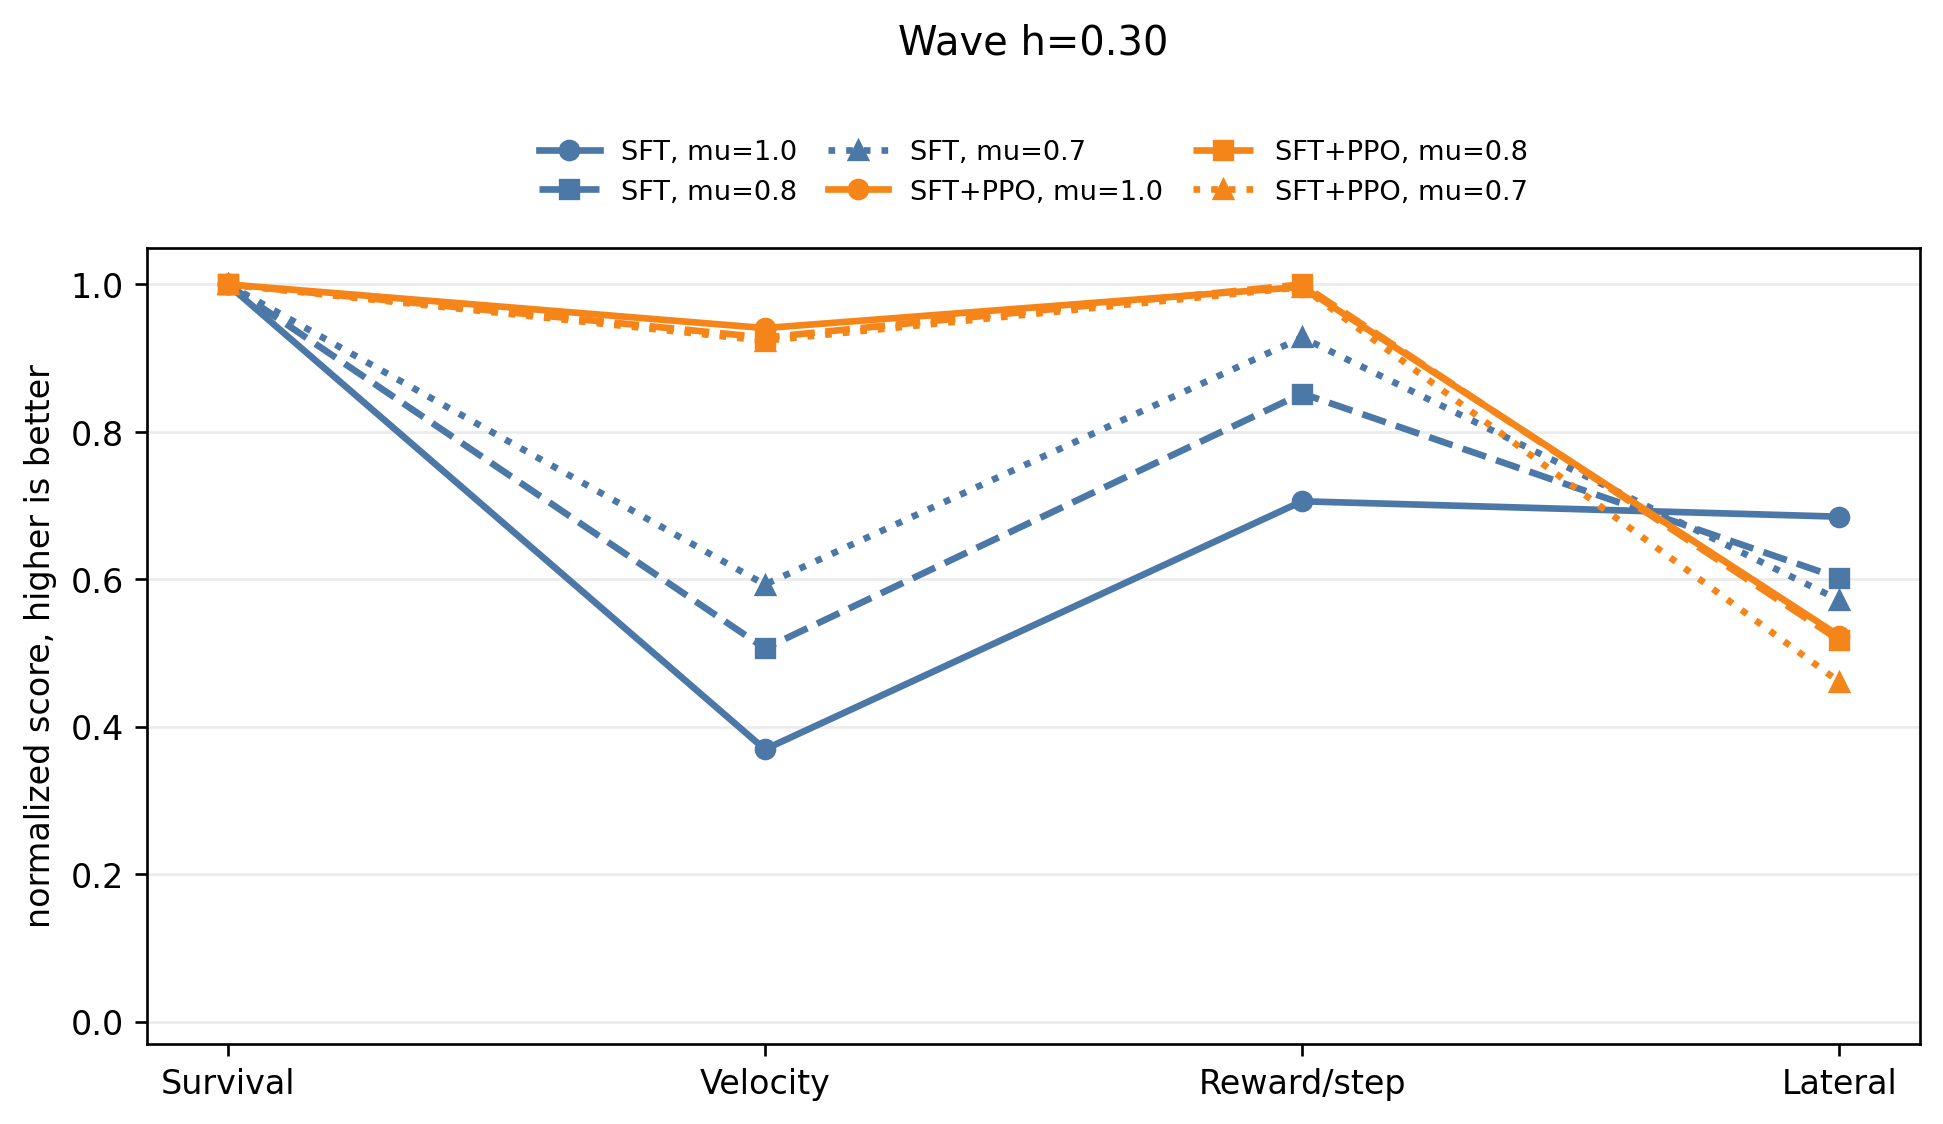
\includegraphics[width=0.98\linewidth]{profile_wave_h030.png}}\\[0.8em]
\subfloat[Irregular h=0.30\label{fig:profile-irregular-030}]{
  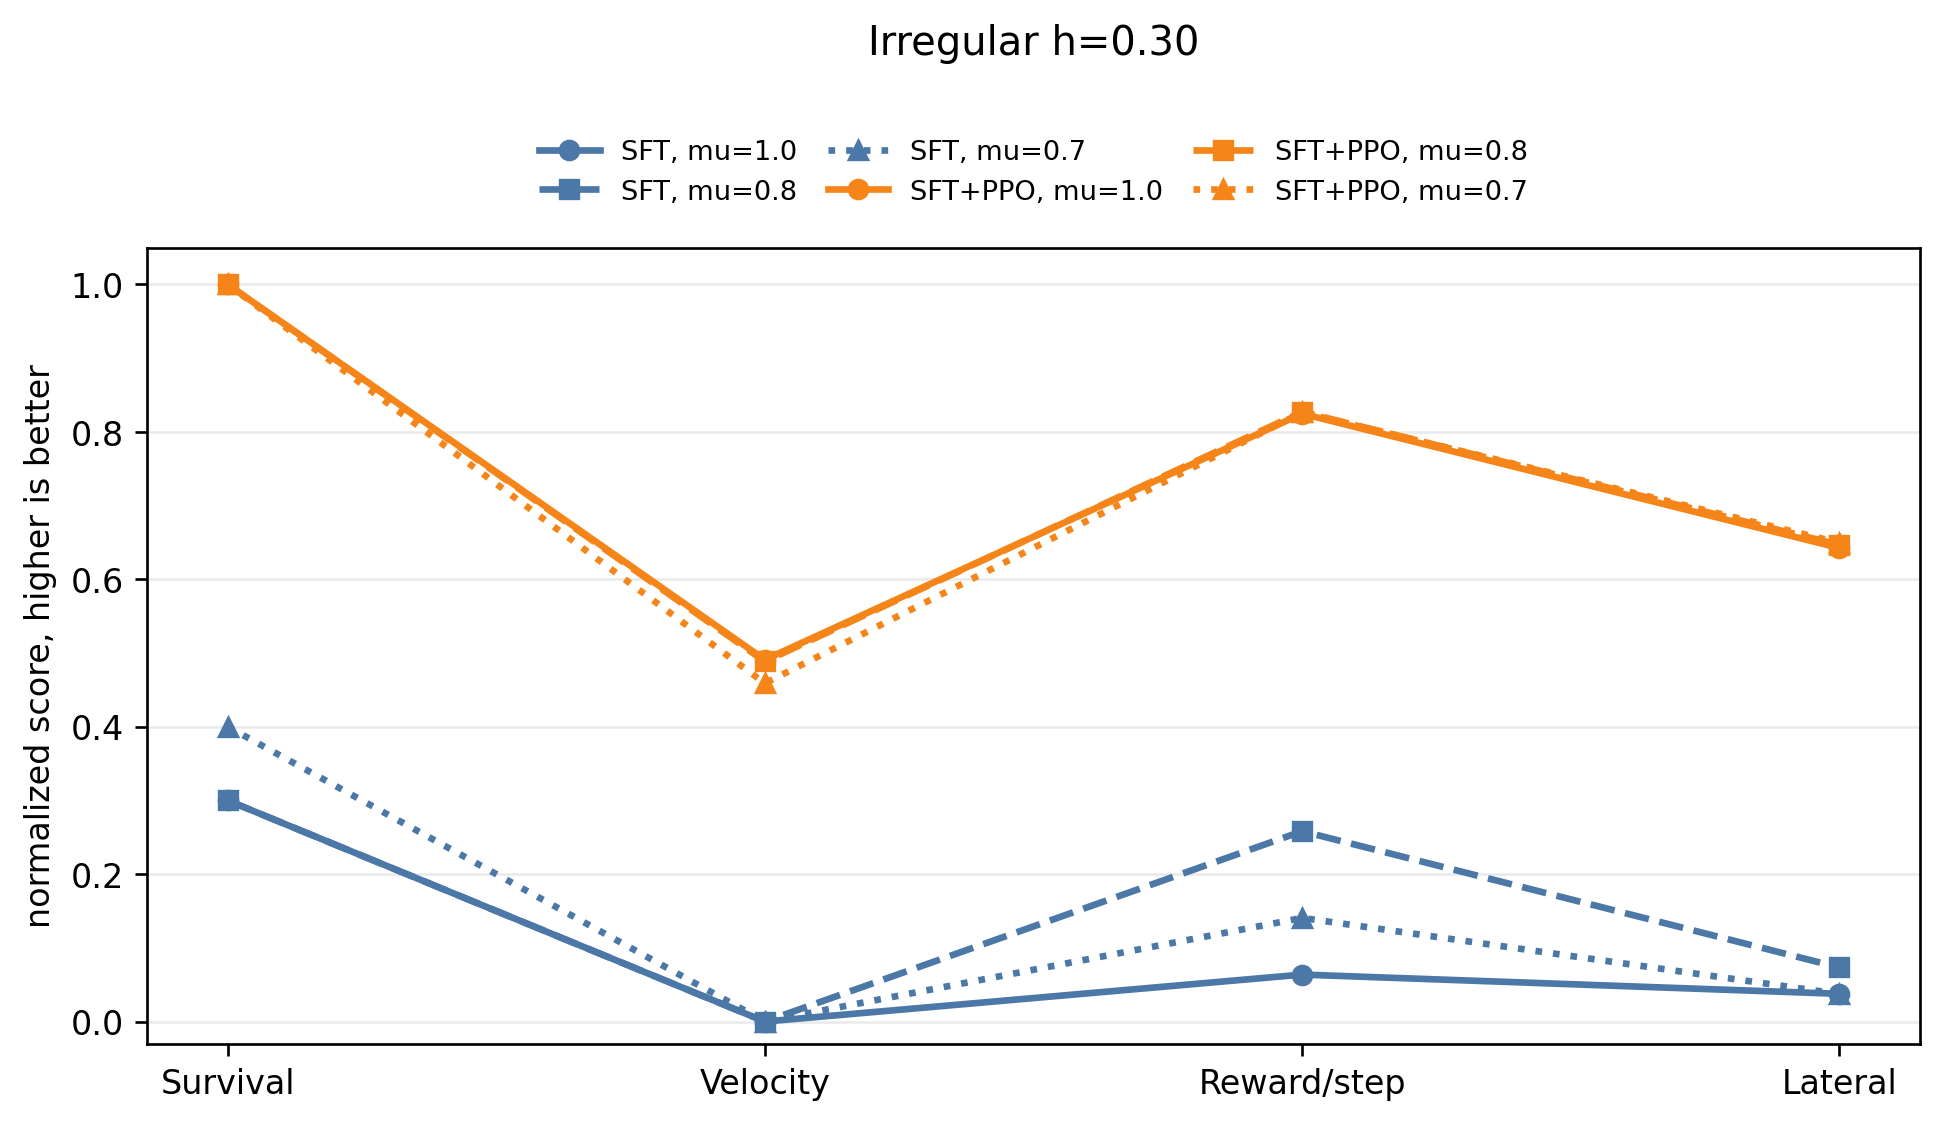
\includegraphics[width=0.98\linewidth]{profile_irregular_h030.png}}\\[0.8em]
\subfloat[Irregular h=0.40\label{fig:profile-irregular-040}]{
  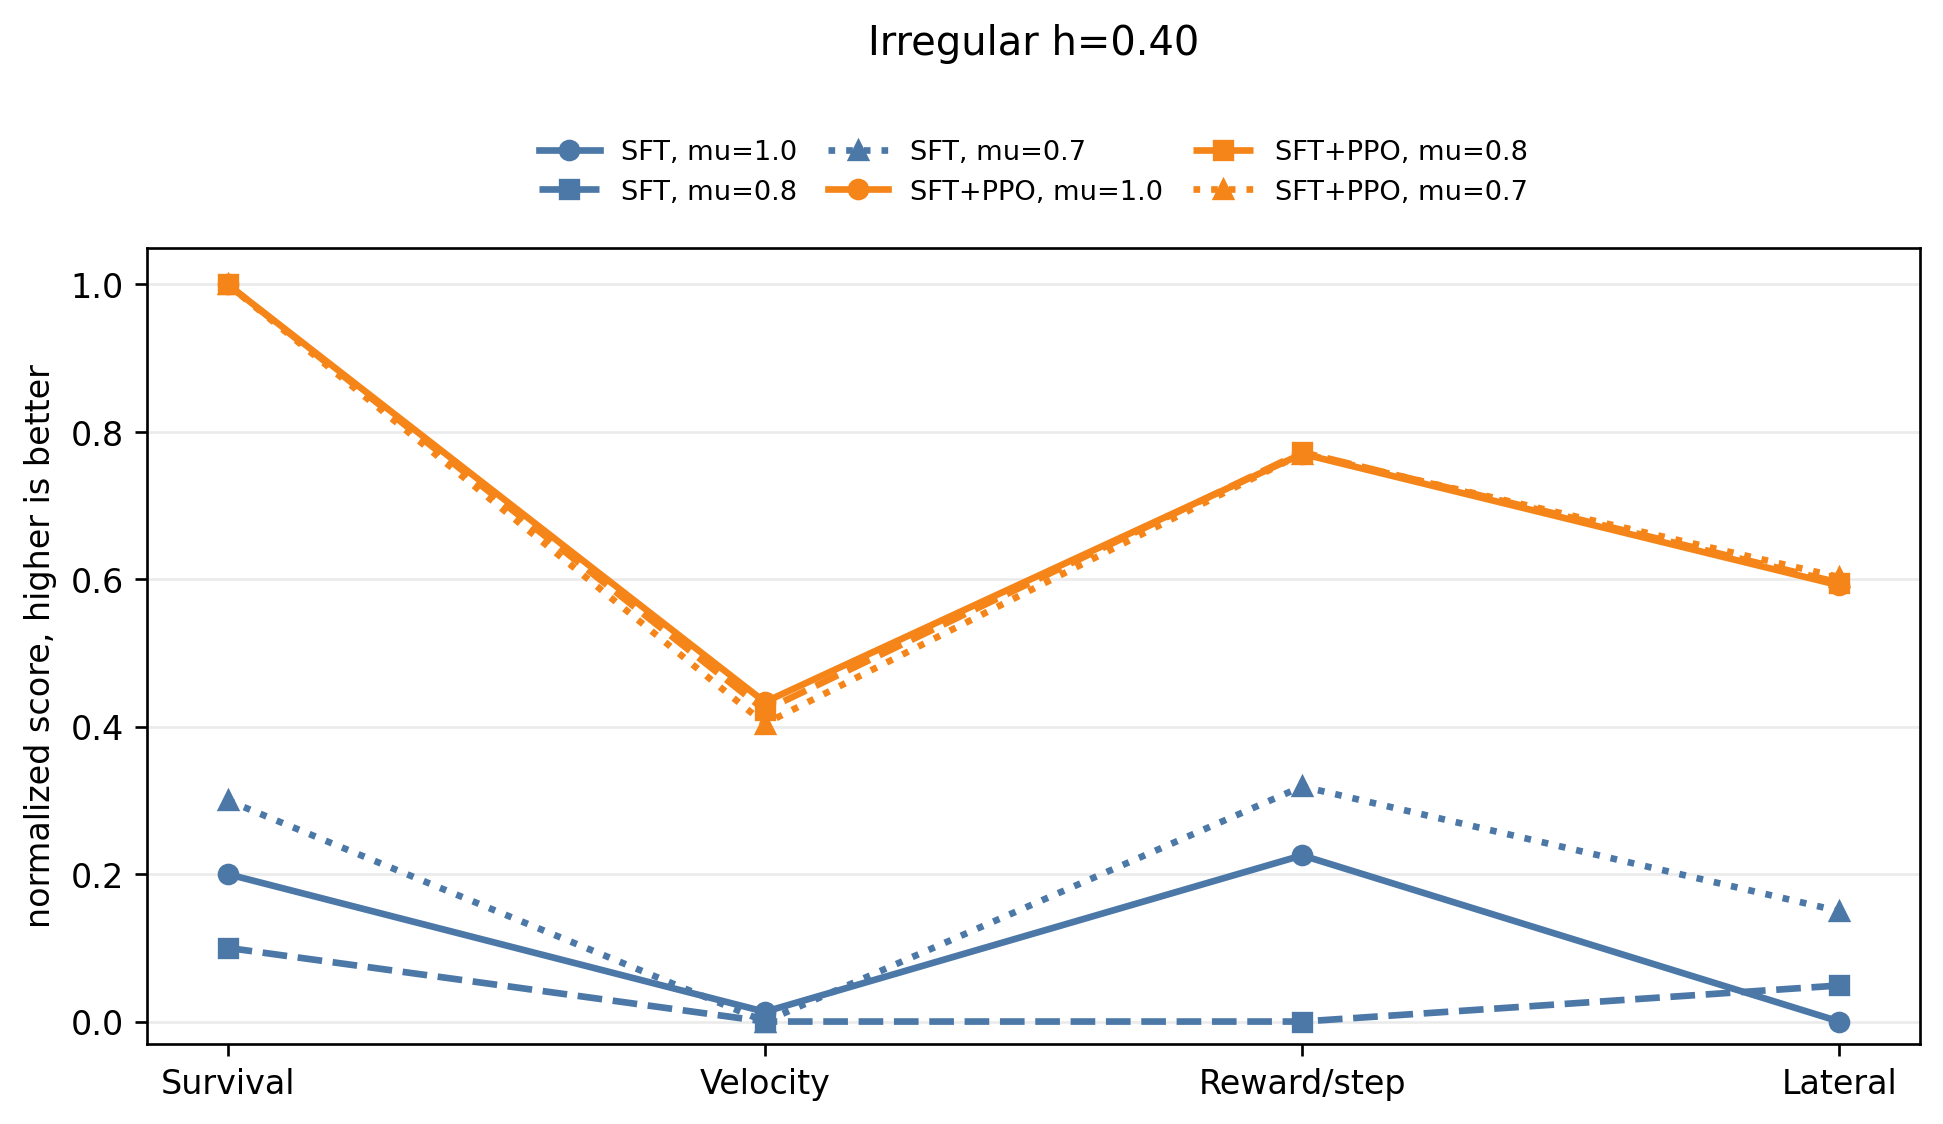
\includegraphics[width=0.98\linewidth]{profile_irregular_h040.png}}
\caption{Profile comparisons with fixed terrain. Each subfigure fixes one terrain and compares six checkpoint--friction combinations.}
\label{fig:profile-by-terrain}
\end{figure}

\begin{figure}[H]
\centering
\subfloat[$\mu=1.0$\label{fig:profile-friction-10}]{
  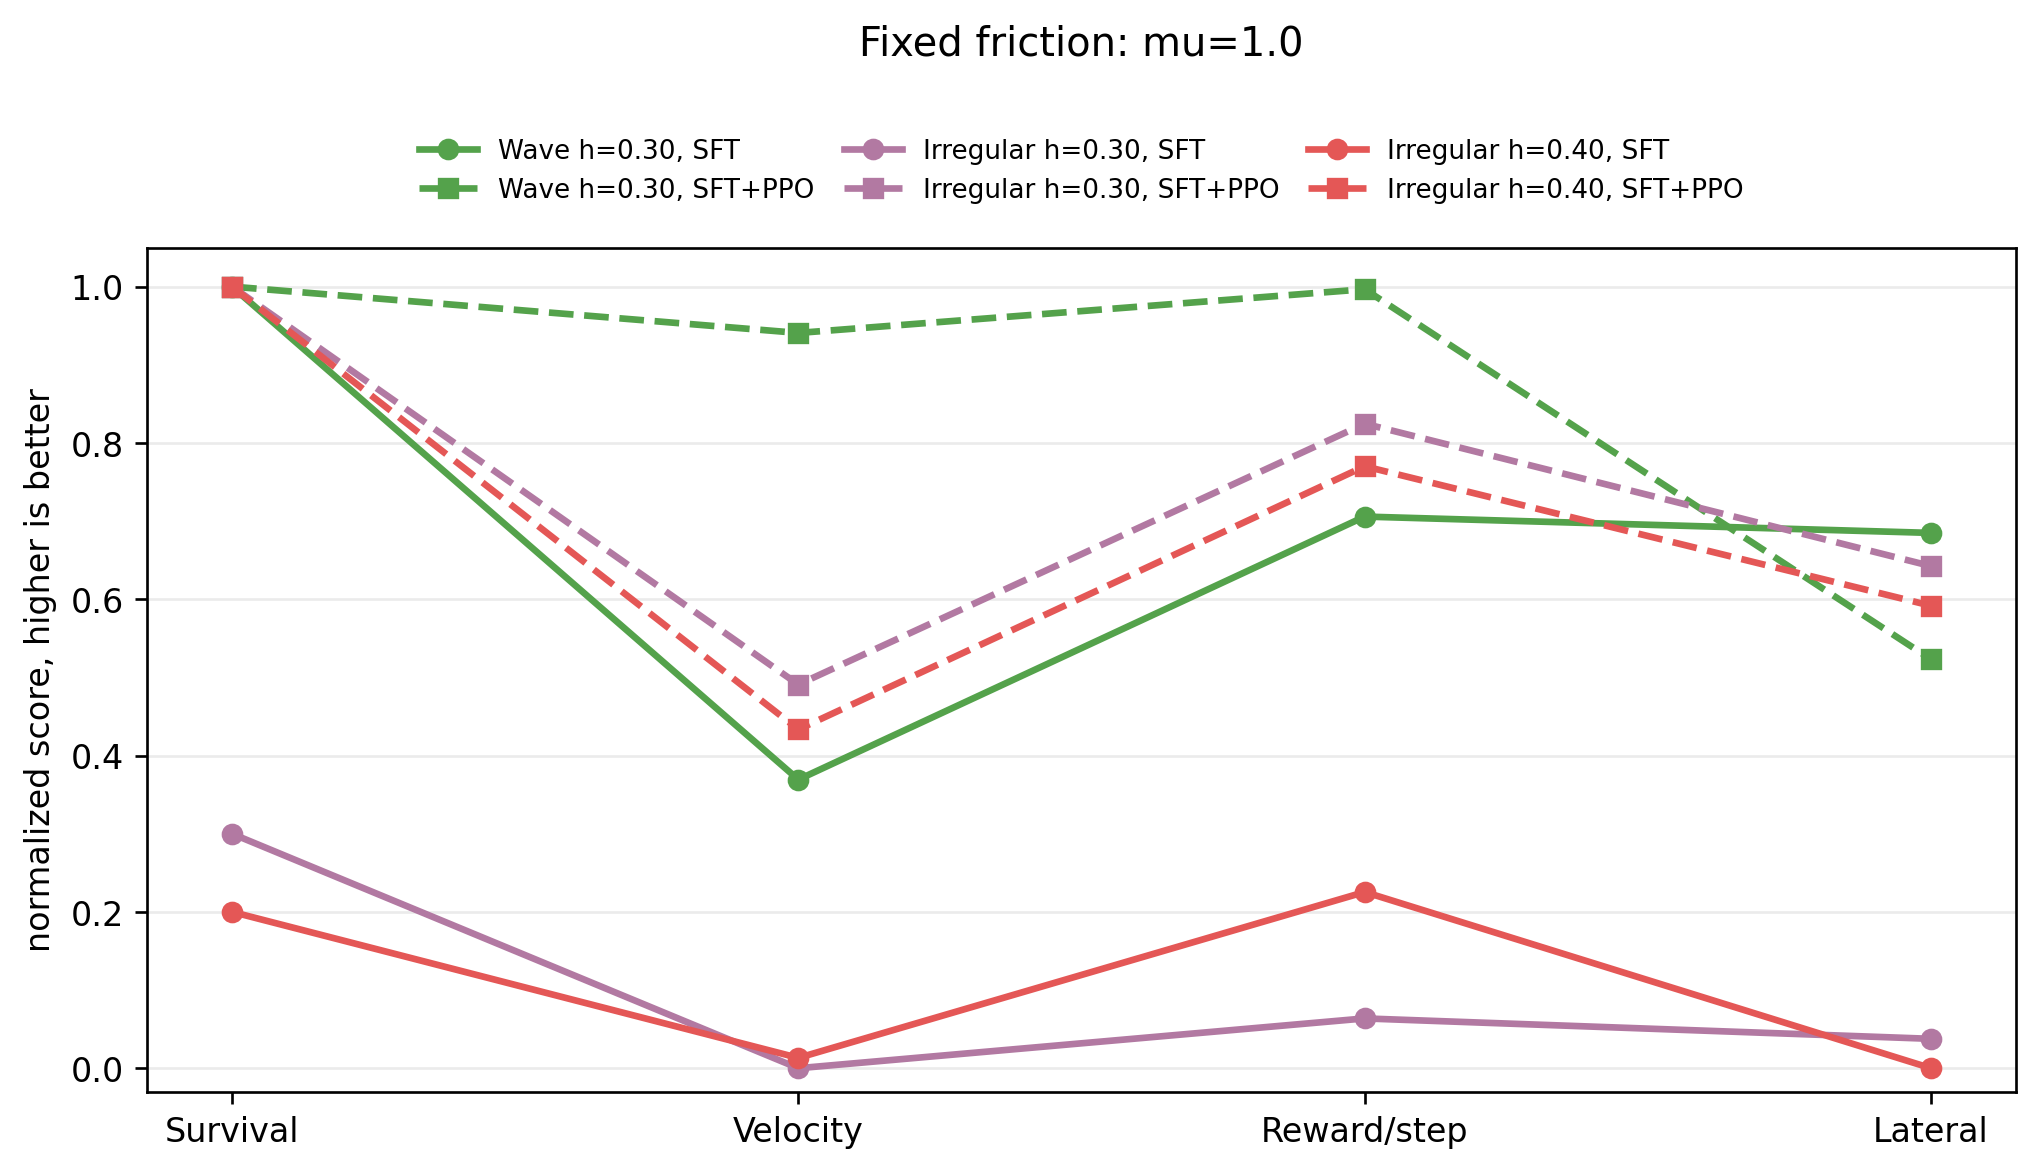
\includegraphics[width=0.98\linewidth]{profile_friction_1p0.png}}\\[0.8em]
\subfloat[$\mu=0.8$\label{fig:profile-friction-08}]{
  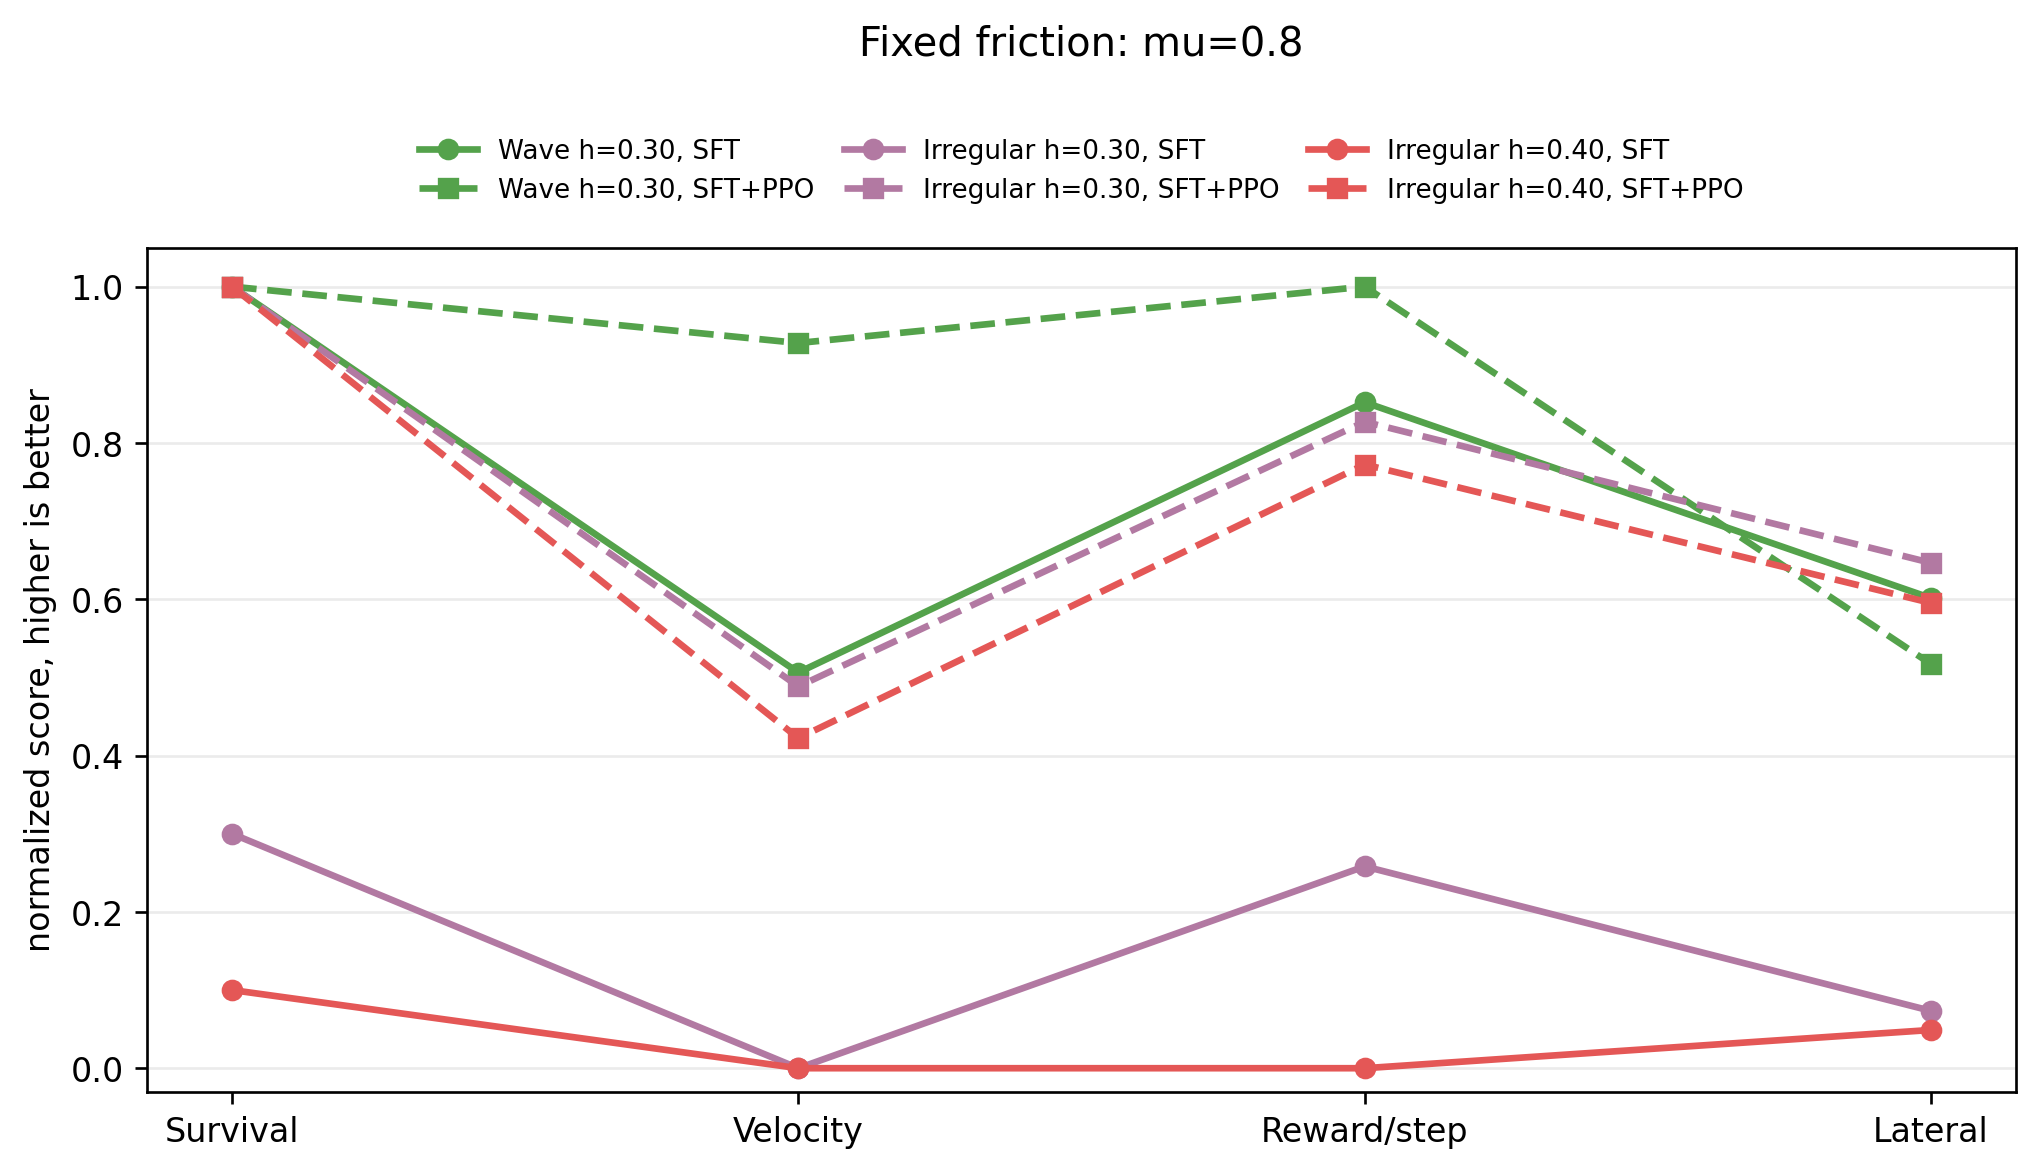
\includegraphics[width=0.98\linewidth]{profile_friction_0p8.png}}\\[0.8em]
\subfloat[$\mu=0.7$\label{fig:profile-friction-07}]{
  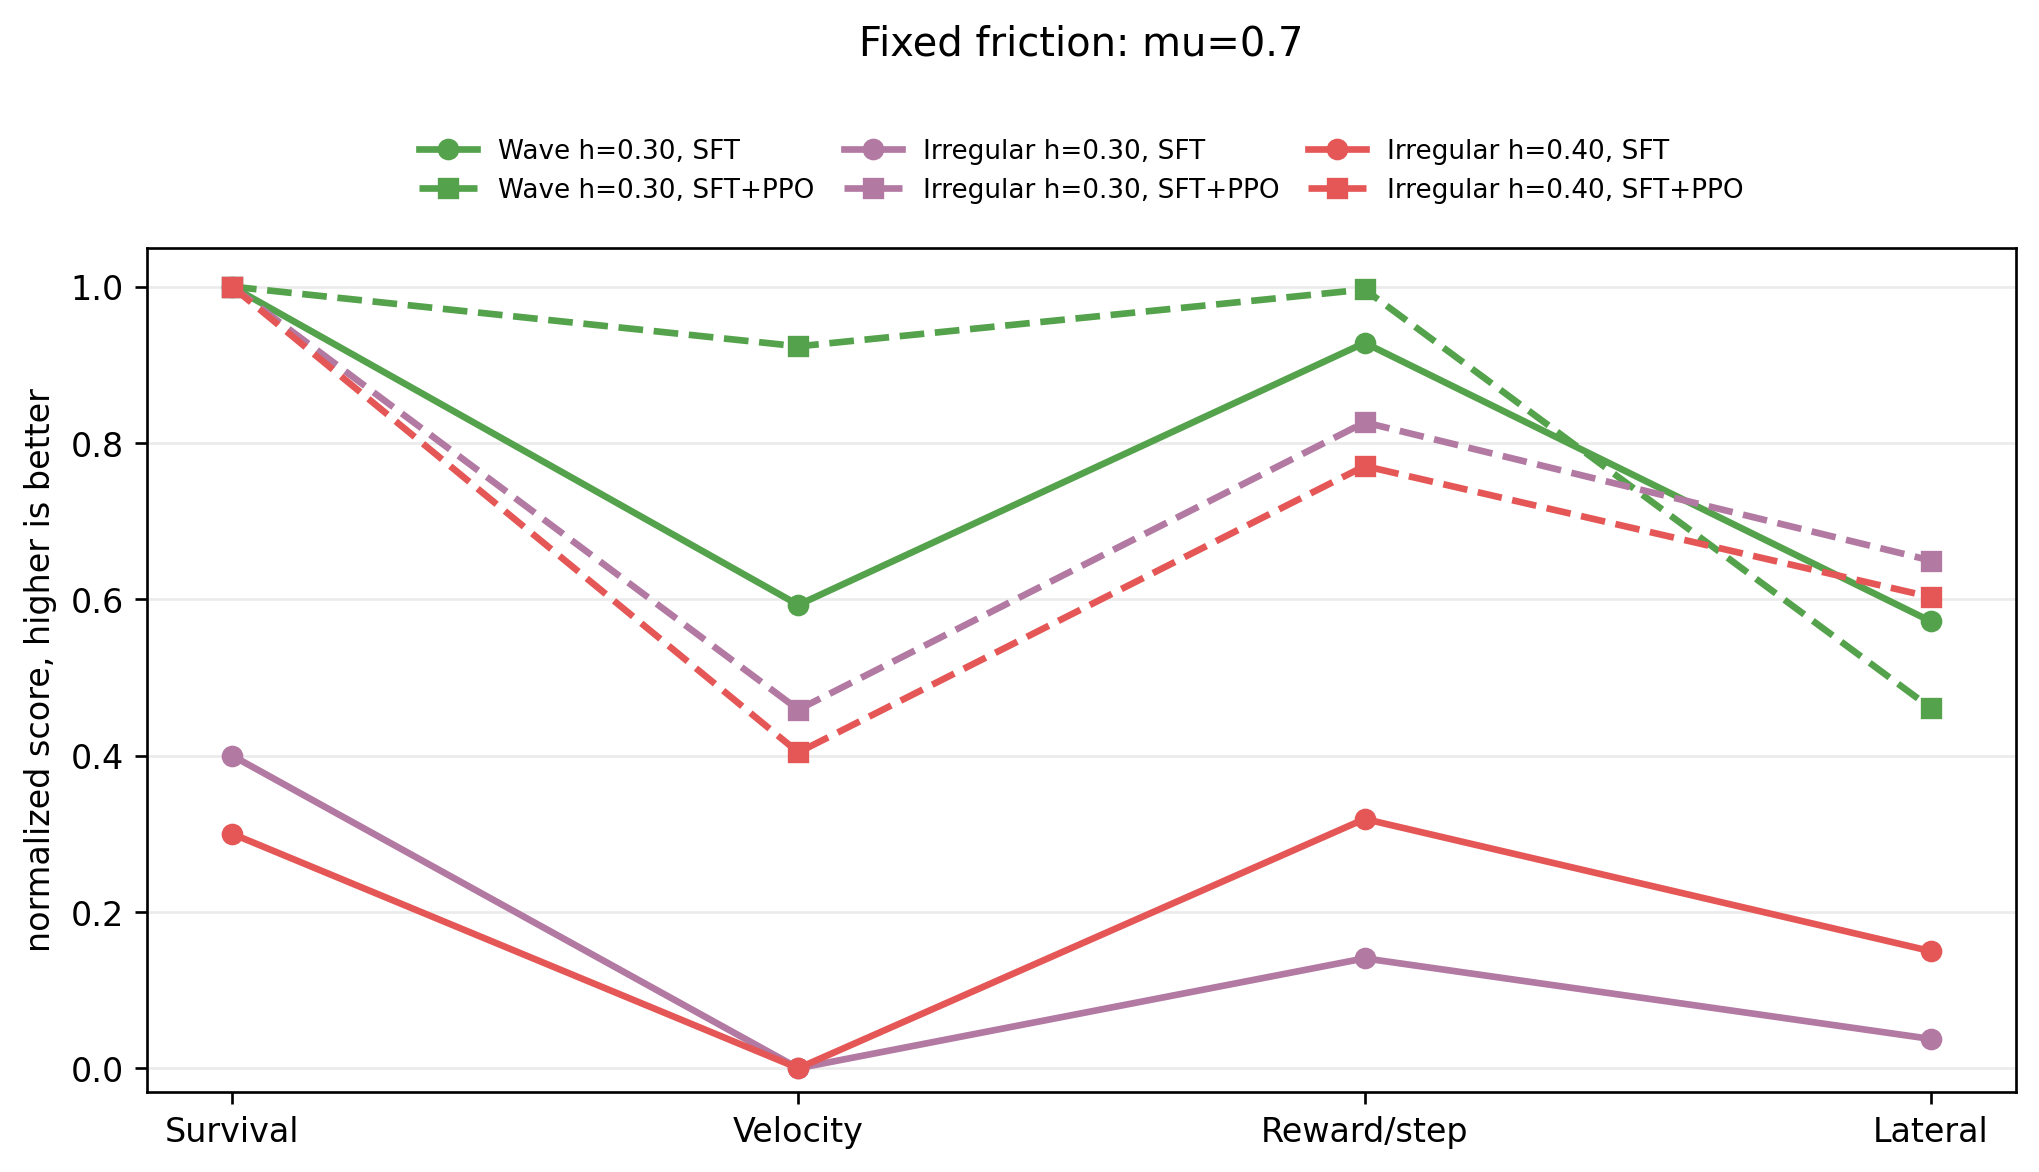
\includegraphics[width=0.98\linewidth]{profile_friction_0p7.png}}
\caption{Profile comparisons with fixed friction. Each subfigure fixes one friction coefficient and compares six terrain--checkpoint combinations.}
\label{fig:profile-by-friction}
\end{figure}

\begin{figure}[H]
\centering
\subfloat[SFT checkpoint\label{fig:profile-checkpoint-sft}]{
  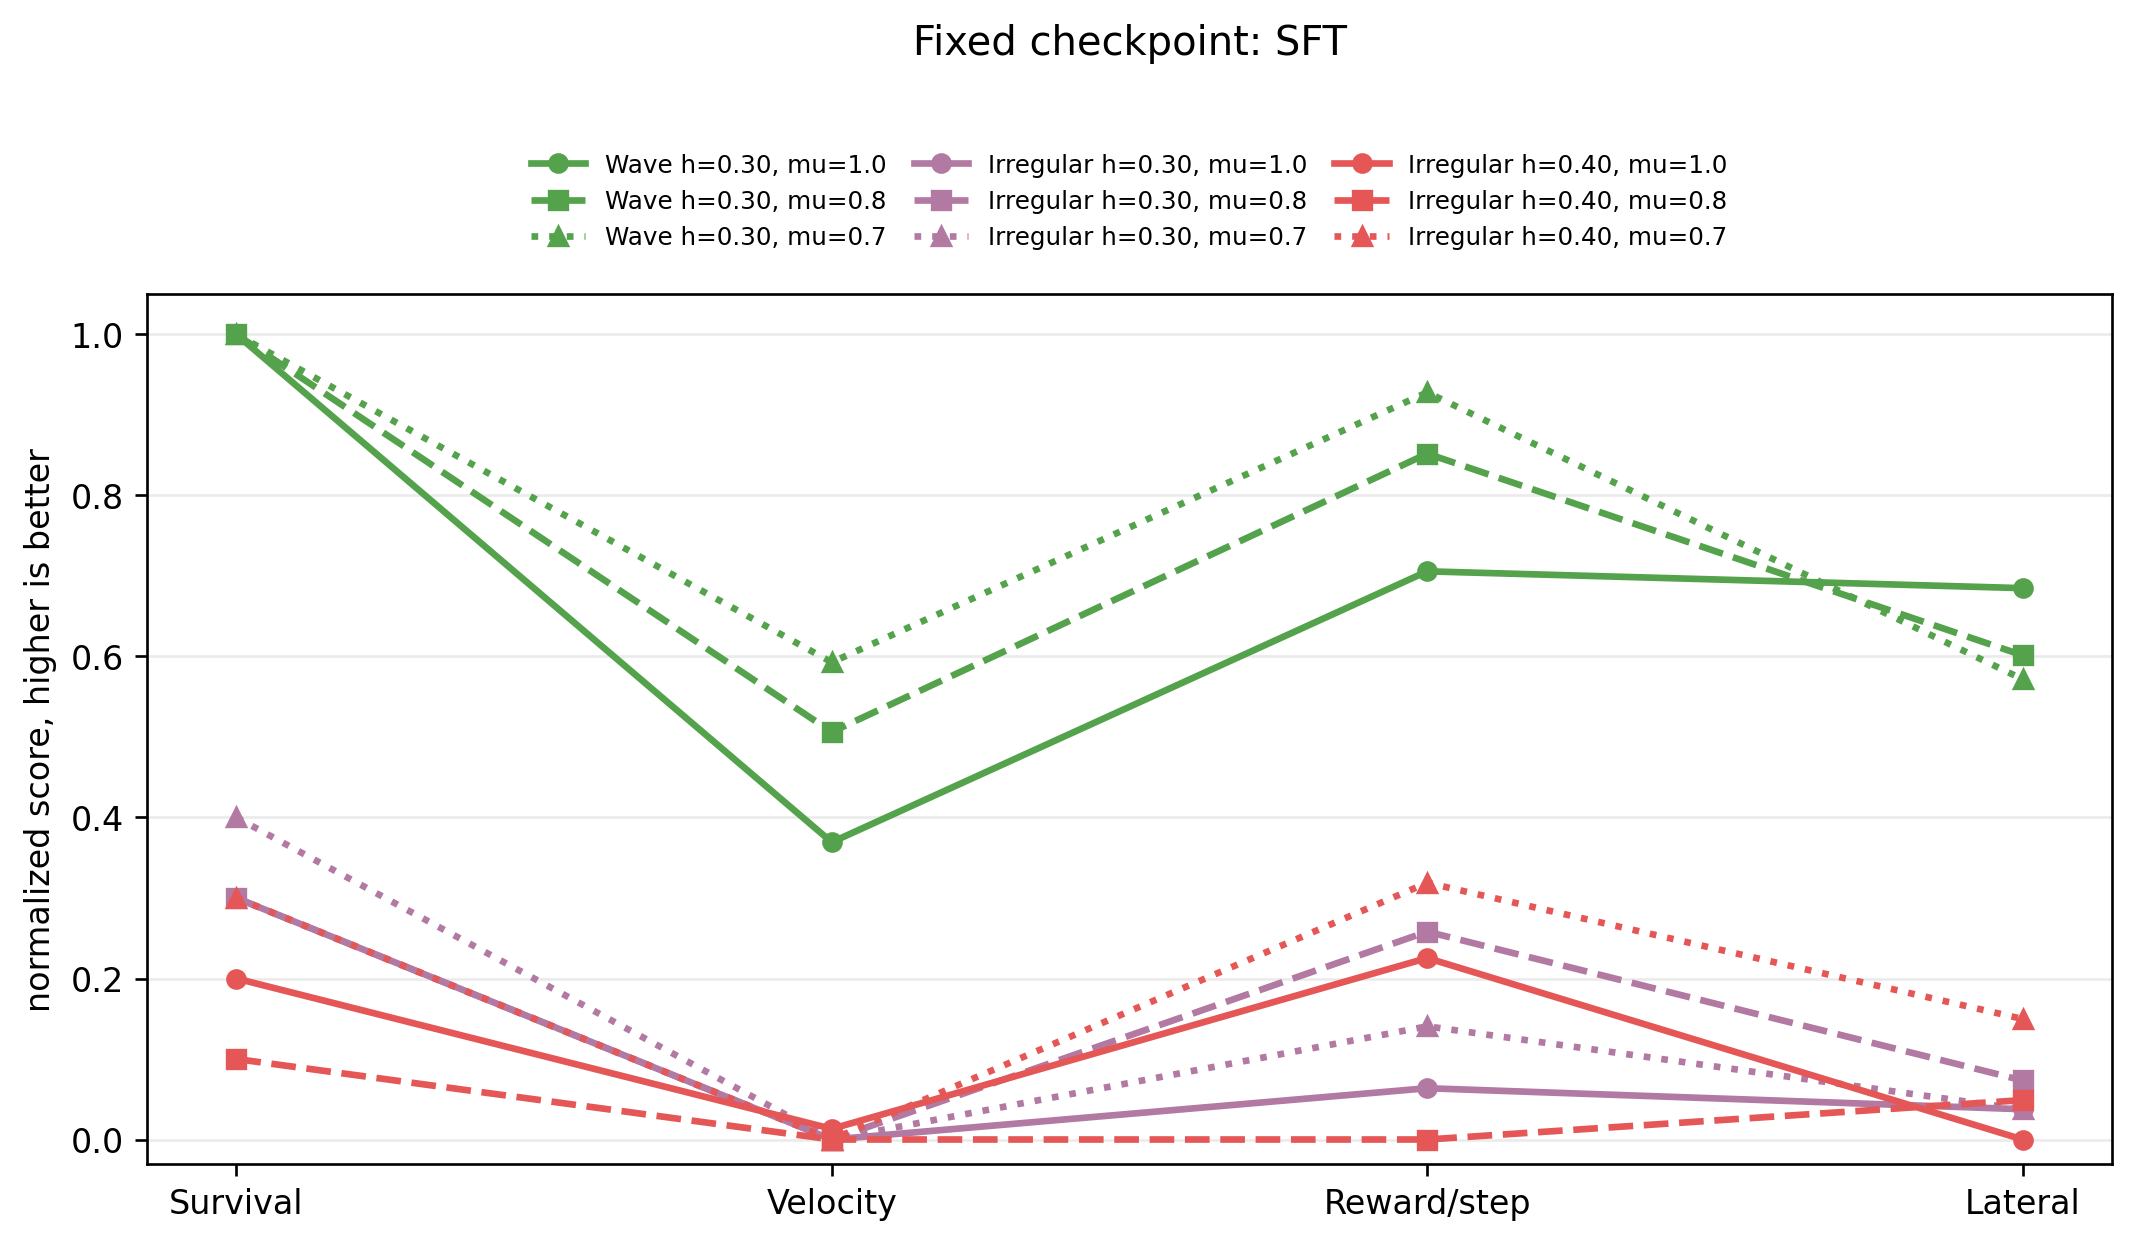
\includegraphics[width=0.98\linewidth]{profile_checkpoint_bc_dog_trot_v3.png}}\\[0.8em]
\subfloat[SFT+PPO checkpoint\label{fig:profile-checkpoint-ppo}]{
  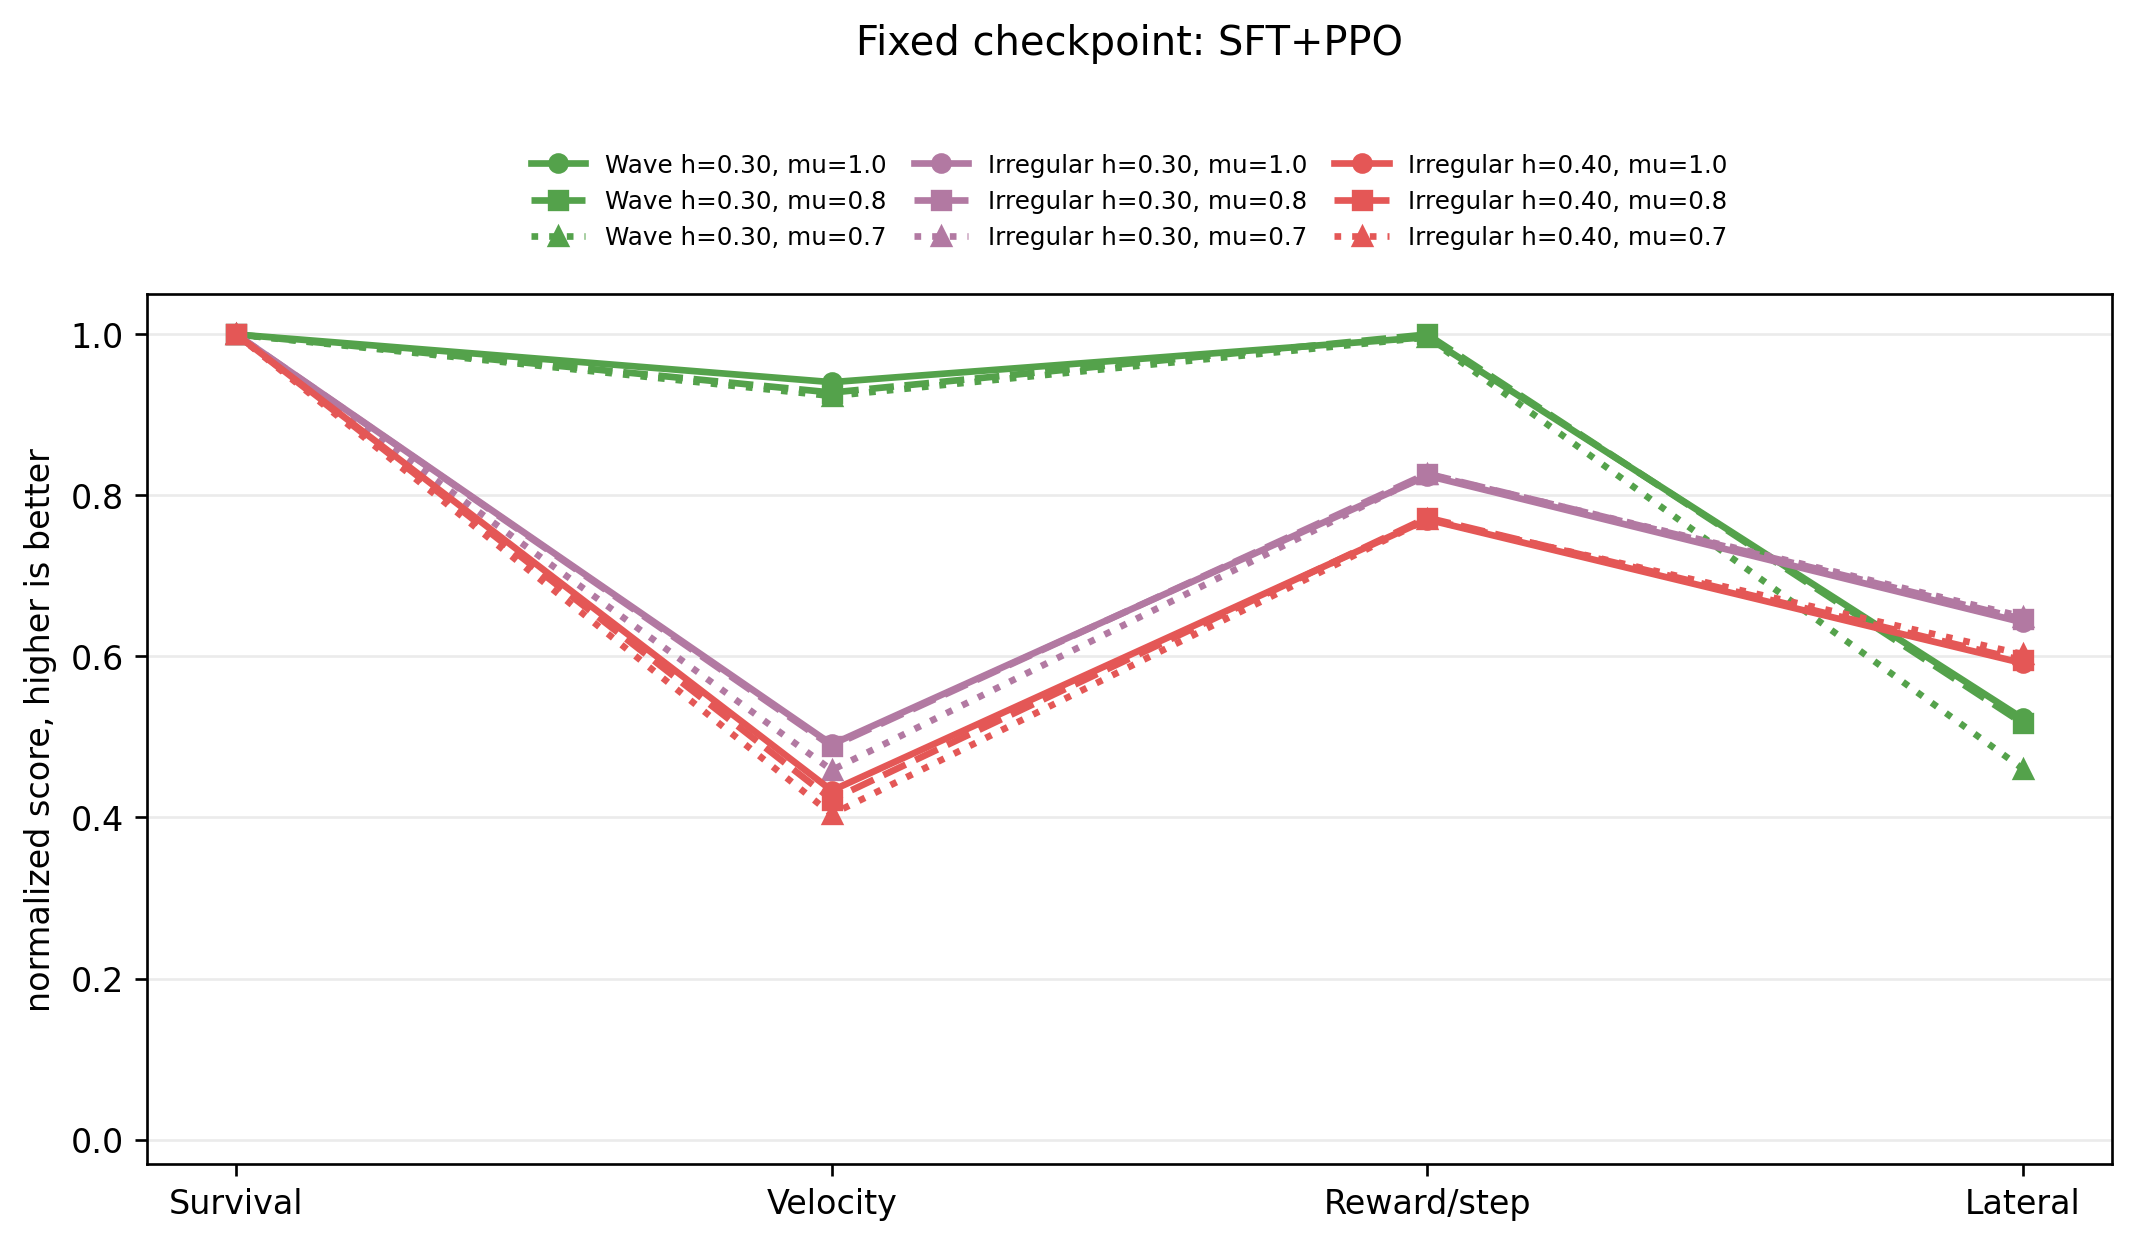
\includegraphics[width=0.98\linewidth]{profile_checkpoint_ppo_after_bc_teacher_v1.png}}
\caption{Profile comparisons with fixed checkpoint. Each subfigure fixes one checkpoint and compares nine terrain--friction combinations.}
\label{fig:profile-by-checkpoint}
\end{figure}
\FloatBarrier


\section{Conclusion}
This project implements a MuJoCo-based Unitree A1 quadruped locomotion system for rough and low-friction terrain. The system combines terrain-aware standing initialization, curriculum-based recovery training, behavior-cloning pretraining from a dog-trot reference motion, and PPO fine-tuning with frozen-teacher action regularization. Experiments show that the resulting policies can recover from disturbances better than the baseline and can walk on both the original wave terrain and a more irregular heightfield. Under reduced friction and stronger terrain perturbations, the walking policy remains stable but slows down.

Future work can improve the project in three directions. First, the recovery and walking checkpoints should be connected by a lightweight classifier or gating module, forming a hierarchical anti-disturbance controller that switches between walking and recovery based on the current state. Second, the teacher regularization can be extended from action-level matching to full reference-trajectory imitation, including joint pose, joint velocity, foot positions, base orientation, and base velocity. Third, training can include stronger domain randomization over terrain geometry, slope, and spatially varying friction, while the reward can include more detailed energy, foot clearance, stride-length, and cadence terms to reduce tiny conservative steps and produce a more natural walking gait.

\begin{thebibliography}{00}
\bibitem{mujoco} E. Todorov, T. Erez, and Y. Tassa, ``MuJoCo: A physics engine for model-based control,'' in \emph{Proc. IEEE/RSJ International Conference on Intelligent Robots and Systems}, 2012, pp. 5026--5033.
\bibitem{ppo} J. Schulman, F. Wolski, P. Dhariwal, A. Radford, and O. Klimov, ``Proximal policy optimization algorithms,'' arXiv preprint arXiv:1707.06347, 2017.
\bibitem{hwangbo2019learning} J. Hwangbo, J. Lee, A. Dosovitskiy, D. Bellicoso, V. Tsounis, V. Koltun, and M. Hutter, ``Learning agile and dynamic motor skills for legged robots,'' \emph{Science Robotics}, vol. 4, no. 26, 2019.
\bibitem{lee2020learning} J. Lee, J. Hwangbo, L. Wellhausen, V. Koltun, and M. Hutter, ``Learning quadrupedal locomotion over challenging terrain,'' \emph{Science Robotics}, vol. 5, no. 47, 2020.
\bibitem{kumar2021rma} A. Kumar, Z. Fu, D. Pathak, and J. Malik, ``RMA: Rapid motor adaptation for legged robots,'' in \emph{Robotics: Science and Systems}, 2021.
\bibitem{margolis2022rapid} G. B. Margolis and P. Agrawal, ``Rapid locomotion via reinforcement learning,'' in \emph{Robotics: Science and Systems}, 2022.
\bibitem{sun2024systematic} B. Sun, S. M. Haris, and R. Ramli, ``A systematic review of deep reinforcement learning for legged robots,'' 2024.
\bibitem{peng2020learning} X. B. Peng, E. Coumans, T. Zhang, T.-W. Lee, J. Tan, and S. Levine, ``Learning agile robotic locomotion skills by imitating animals,'' in \emph{Robotics: Science and Systems}, 2020.
\bibitem{sb3} A. Raffin, A. Hill, A. Gleave, A. Kanervisto, M. Ernestus, and N. Dormann, ``Stable-Baselines3: Reliable reinforcement learning implementations,'' \emph{Journal of Machine Learning Research}, vol. 22, no. 268, pp. 1--8, 2021.
\bibitem{unitree} Unitree Robotics, ``A1 quadruped robot,'' 2020. [Online]. Available: \url{https://www.unitree.com/}
\end{thebibliography}

\end{document}
